\documentclass[border=2pt,tikz]{standalone}

\usepackage{physics}

\usepackage{amsfonts,amssymb,amsmath}
\usepackage{tikz-cd}
\usepackage{tikz}
\usepackage{mathdots}
\usepackage{yhmath}
\usepackage{cancel}
\usepackage{color}
\usepackage{siunitx}
\usepackage{array}
\usepackage{multirow}
\usepackage{amssymb}
\usepackage{gensymb}
\usepackage{tabularx}


\usetikzlibrary{decorations.pathmorphing}

\begin{document}
% Gradient Info

\tikzset{every picture/.style={line width=0.75pt}} %set default line width to 0.75pt

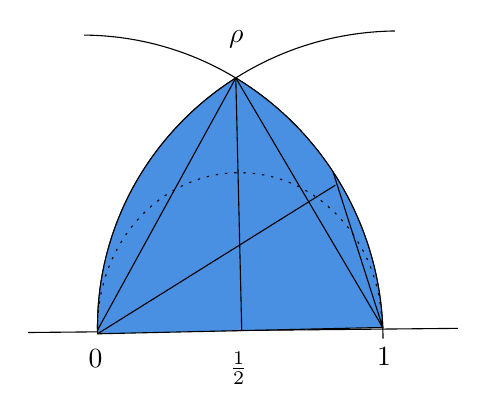
\begin{tikzpicture}[x=0.75pt,y=0.75pt,yscale=-1,xscale=1]
%uncomment if require: \path (0,300); %set diagram left start at 0, and has height of 300

%Straight Lines [id:da07964668391959173]
\draw    (187.5,206) -- (394.5,204) ;
%Shape: Arc [id:dp22858111461352082]
\draw  [draw opacity=0] (214.38,62.7) .. controls (293.37,63.3) and (357.63,127.95) .. (358.43,208.26) .. controls (358.43,208.47) and (358.43,208.68) .. (358.43,208.89) -- (213.32,209.65) -- cycle ; \draw   (214.38,62.7) .. controls (293.37,63.3) and (357.63,127.95) .. (358.43,208.26) .. controls (358.43,208.47) and (358.43,208.68) .. (358.43,208.89) ;
%Shape: Arc [id:dp38540768514578816]
\draw  [draw opacity=0] (220.92,206.64) .. controls (220.91,206.02) and (220.9,205.41) .. (220.89,204.79) .. controls (220.11,126.13) and (284.21,61.71) .. (364.15,60.72) -- (365.99,203.4) -- cycle ; \draw   (220.92,206.64) .. controls (220.91,206.02) and (220.9,205.41) .. (220.89,204.79) .. controls (220.11,126.13) and (284.21,61.71) .. (364.15,60.72) ;
%Shape: Path Data [id:dp8914637131357663]
\draw  [fill={rgb, 255:red, 74; green, 144; blue, 226 }  ,fill opacity=1 ] (220.9,204.8) .. controls (220.39,153.93) and (247.02,109.03) .. (287.51,83.37) .. controls (328.3,108.01) and (356.21,152.36) .. (358.3,203.57) -- (220.93,206.62) .. controls (220.91,206.01) and (220.9,205.41) .. (220.9,204.8) -- cycle ;
%Straight Lines [id:da16871124312897057]
\draw    (287.51,83.37) -- (290.36,204.86) ;
%Straight Lines [id:da7507794574246773]
\draw    (335.5,135) -- (220.93,206.62) ;
%Straight Lines [id:da5854117367826361]
\draw    (334.37,128.67) -- (358.3,203.57) ;
%Straight Lines [id:da4757673542202314]
\draw    (358.3,203.57) -- (287.51,83.37) ;
%Straight Lines [id:da4839886084785838]
\draw    (220.9,204.8) -- (287.51,83.37) ;
%Shape: Arc [id:dp7626930956428462]
\draw  [draw opacity=0][dash pattern={on 0.84pt off 2.51pt}] (220.92,205.45) .. controls (220.91,205.08) and (220.9,204.7) .. (220.9,204.33) .. controls (220.57,163.03) and (250.97,129.31) .. (288.8,129) .. controls (326.2,128.7) and (356.87,161.18) .. (357.88,201.83) -- (289.4,203.78) -- cycle ; \draw  [dash pattern={on 0.84pt off 2.51pt}] (220.92,205.45) .. controls (220.91,205.08) and (220.9,204.7) .. (220.9,204.33) .. controls (220.57,163.03) and (250.97,129.31) .. (288.8,129) .. controls (326.2,128.7) and (356.87,161.18) .. (357.88,201.83) ;

% Text Node
\draw (283,59.4) node [anchor=north west][inner sep=0.75pt]    {$\rho $};
% Text Node
\draw (215.32,213.05) node [anchor=north west][inner sep=0.75pt]    {$0$};
% Text Node
\draw (354.32,212.05) node [anchor=north west][inner sep=0.75pt]    {$1$};
% Text Node
\draw (283.32,214.05) node [anchor=north west][inner sep=0.75pt]    {$\frac{1}{2}$};


\end{tikzpicture}
\end{document}
